\selectlanguage{italian}%

\section{Soluzione}


\subsection{Schematici 	\label{Dati ripple carry}}

\begin{figure}[H]
	\centering
	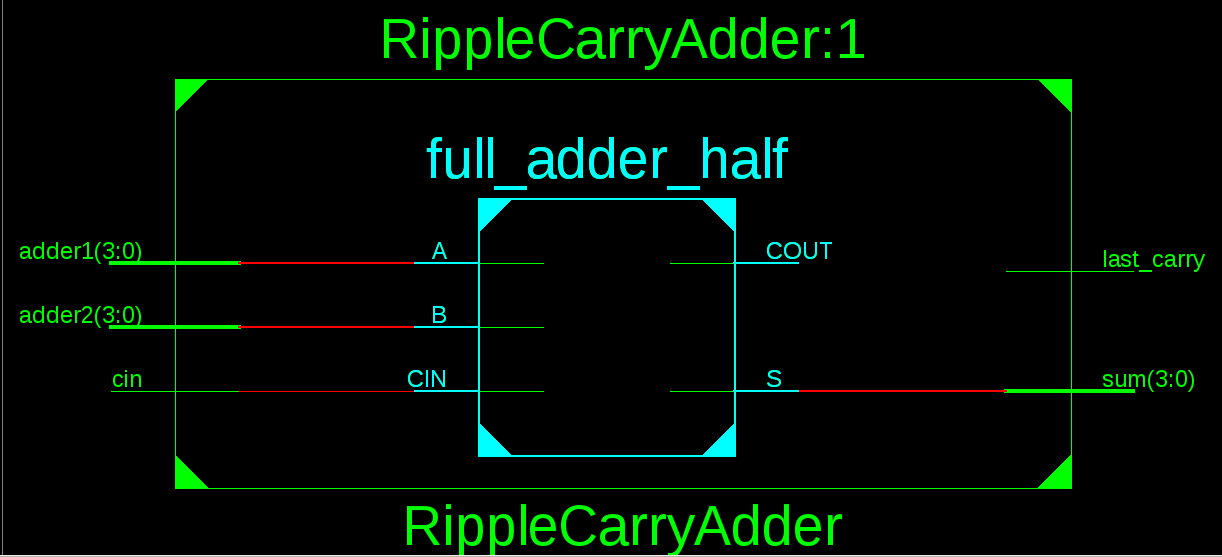
\includegraphics[scale=0.4]{esercizio08/images/ripple_carry_adder.png}
	\caption{Ripple Carry Adder}
\end{figure}

Per realizzare il circuito si � ricorsi al costrutto for generate,
per colleggare i vari full adder per far s� che i riporti generati
dal full adder precedente vengano propagati al successivo, purtroppo
dallo schematico non � evidente, perch� i costrutti di questo tipo
quando viene chiesto ad ISE di creare lo schematico non lo espande
mostrando tutti i singoli full\_adder, ma ne crea uno solo che per�
ha in ingresso ed uscita un vettore di bit.

\begin{table}[H]

\noindent\begin{minipage}[t]{1\columnwidth}%
\begin{tabular}{|c|c|c|c|}
\hline 
Numero di bit operandi & Numero di slice & Numero di four LUT & Tempo di calcolo\tabularnewline
\hline 
\hline 
4 & 6 & 8 & 7,225 ps\tabularnewline
\hline 
8 & 12 & 16 & 7,735 ps\tabularnewline
\hline 
16 & 24 & 32 & 9,358 ps\tabularnewline
\hline 
32 & 48 & 64 & 9,985 ps\tabularnewline
\hline 
\end{tabular}%
\end{minipage}

\end{table}

Secondo le formule dell' area e del ritardo, l' area � pari a 5$n$
(dove $n$ indica il numero di full-adder) , ed 2$\delta$$n$ per
il ritardo, la realizzazione per FPGA invece presenta dimensioni e
ritardi diversi, difatti l' area raddoppia se raddoppiano il numero
di bit per la somma, molto probabilmente perch� utilizzer� ogni slice
come un full adder, invece il tempo di calcolo all' aumentare del
numero di bit cresce ma meno che linearmente, determinante dal fatto
che il sintetizzatore riuscir� a disporre le slice molto vicine tra
di loro e il tempo di propagazione dei riporti diverr� molto piccolo,
si nota per� che da 8 a 16 bit il tempo di calcolo incrementa di una
quantit� maggiore rispetto al passaggio da a 4 a 8 o da 16 a 32, perch�
le connessioni non avvengono tra CLB vicini tra loro, per determinare
il tempo si � scelto come input sempre il massimo valore accettabile
in ingresso.

Non � stato possibile testare il componente con numero di bit di operandi
a 64 bit, poich� quando si cerca di mappare sulla scheda i vari pin
di ingresso e di uscita dell ' addizionatore, questa operazione non
riesce, una soluzione sarebbe quella di evitare che I/O venga mappato,
per� ISE ci avverte che i tempi di propagazione potrebbero essere
non veritieri, allora si potrebbe utilizzare un altro componente per
far passare gli input non contemporaneamente all' addizionatore, ma
l' area del dispositivo verrebbe influenzata da tutte le connessioni
che occorrono per questo dispositivo e ci potrebbero essere delle
ottimizzazioni che minimizzano l' area.

\subsection{Codice}

\href{run:progetti/RippleCarryAdder/RippleCarryAdder.xise}{Ripple Carry Adder ISE}\selectlanguage{italian}%

